\section{Wstępne Badania}
\label{wstepne_badania}

	\subsection{Testy holonomiczności bazy}
		Aby móc prowadzić prace nad platformą holonomiczną należy najpierw upewnić się, że jej sterownik działa prawidłowo.
		W celu weryfikacji przetestowano symulator z pomocą skryptu ustawiającego prędkości w taki sposób, aby robot jechał po okręgu. 
		Na temat \textit{/cmd\_vel} były pubikowane odpowiednie prędkości w osiach  \textit{x} oraz \textit{y} bazy jezdnej.
		Ilustracja poniższa pokazuje, że sterownik działa bez zarzutu i sterując wspomnianymi prędkościami można prowadzić bazę w dowolnym kierunku.
		
		\begin{figure}
			\centering
			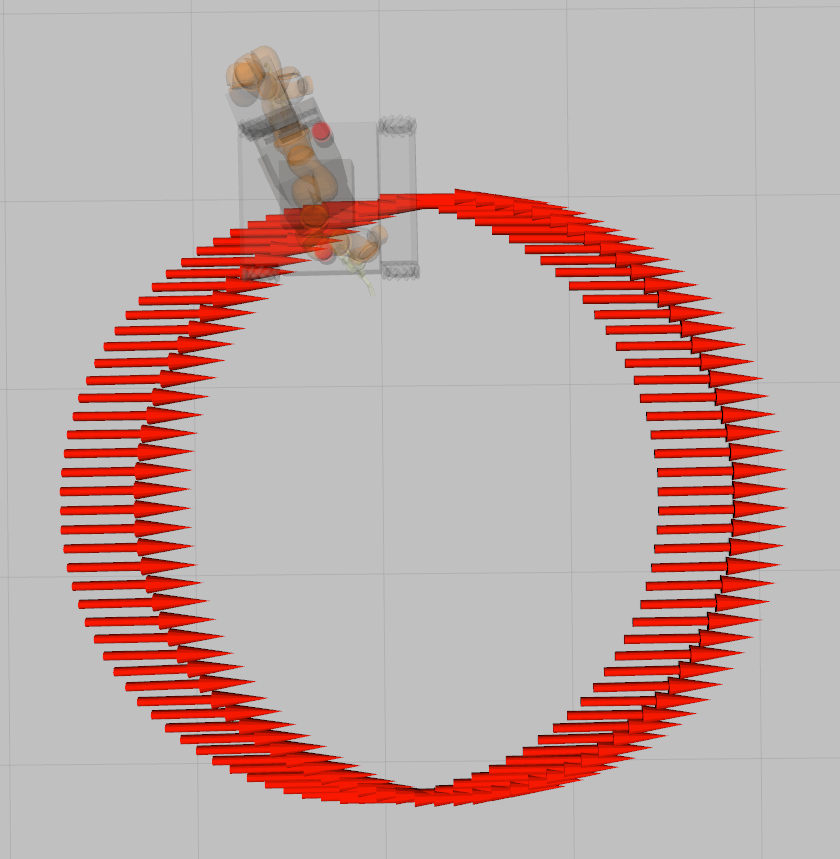
\includegraphics[width=\linewidth]{imgs/wstepne_badania/circle.png}
			\caption{ruch po okręgu ze stałą orientacją względem świata}
			\label{fig:tf}
		\end{figure}

		Kierunek strzał oznacza, że orientacja bazy podczas ruchu nie ulegała zmianie, natomiast wszystkie punkty układają się w pełen okrąg.
		
		Następnym testem, który został przeprowadzony, był test planera globalnego i lokalnego udostępnionych razem z platformą.
		Ze względu na nacisk położony na holonomiczny ruch bazy poświęciłem więcej uwagi algorytmowi planowania lokalnego, plan globalny był jedynie weryfikowany przez sprawdzenie, czy została wytyczona ścieżka.
		Zadaniem robota było przejechanie z punktu o współrzędnych $[1.0 ,2.0]$ do współrzędnych $[2.0, 0.0]$.
		

		\begin{figure}[h!]
 			 \centering
  			\begin{subfigure}[b]{0.4\linewidth}
   				 \includegraphics[width=\linewidth]{imgs/wstepne_badania/plan.png}
    				\caption{plan globalny i lokalny}
  			\end{subfigure}
  			\begin{subfigure}[b]{0.4\linewidth}
    				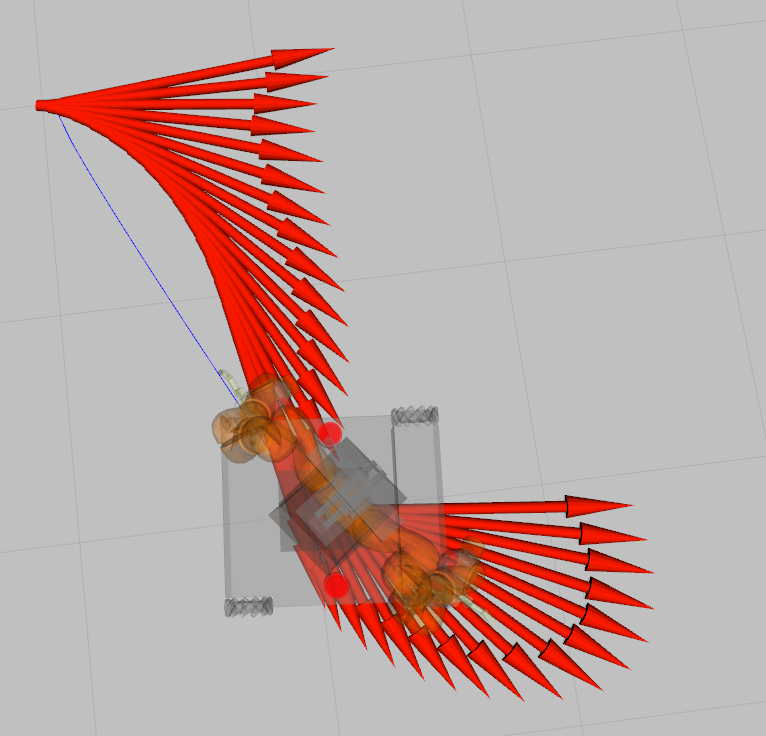
\includegraphics[width=\linewidth]{imgs/wstepne_badania/path.png}
   				 \caption{trajektoria ruchu}
  			\end{subfigure}
  			\caption{The same cup of coffee. Two times.}
 			 \label{fig:plan}
		\end{figure}

		Na pierwszym rysunku z \ref{fig:plan} pokazano, jak plan globalny prawidłowo wyznaczył najkrótszą ścieżkę do punktu docelowego. 
		Natomiast ścieżka algorytmu lokalnego pokazuje, że robot jest traktowany jako baza różnicowa, co ostatecznie dowodzi trajektoria ruchu widoczna na drugiej ilustracji.
		
	\subsection{Budowanie mapy}
		
		W obecnej chwili do budowy mapy można wykorzystywać jedynie pojedynczy czujnik laserowy znajdujący się po lewej lub po prawej stronie bazy jezdnej.
		Jest również zaimplementowana projekcja mapy zajętości generowanej przez kamerę Kinect na płaszczyznę dwuwymiarową, jednak nie została jeszcze ona zintegrowana z modułem odpowiedzialnym za tworzenie map statycznych, na chwilę pisania tego rozdziału budowanie mapy opiera się tylko na pojedymczym skanerze laserowym.
		Na ilustracjach \ref{fig:scan} pokazano, jak na mapę lokalną został zrzutowany fragment wystającego blatu stolika.
			
			
		\begin{figure}[h!]
 			 \centering
  			\begin{subfigure}[h]{\linewidth}
   				 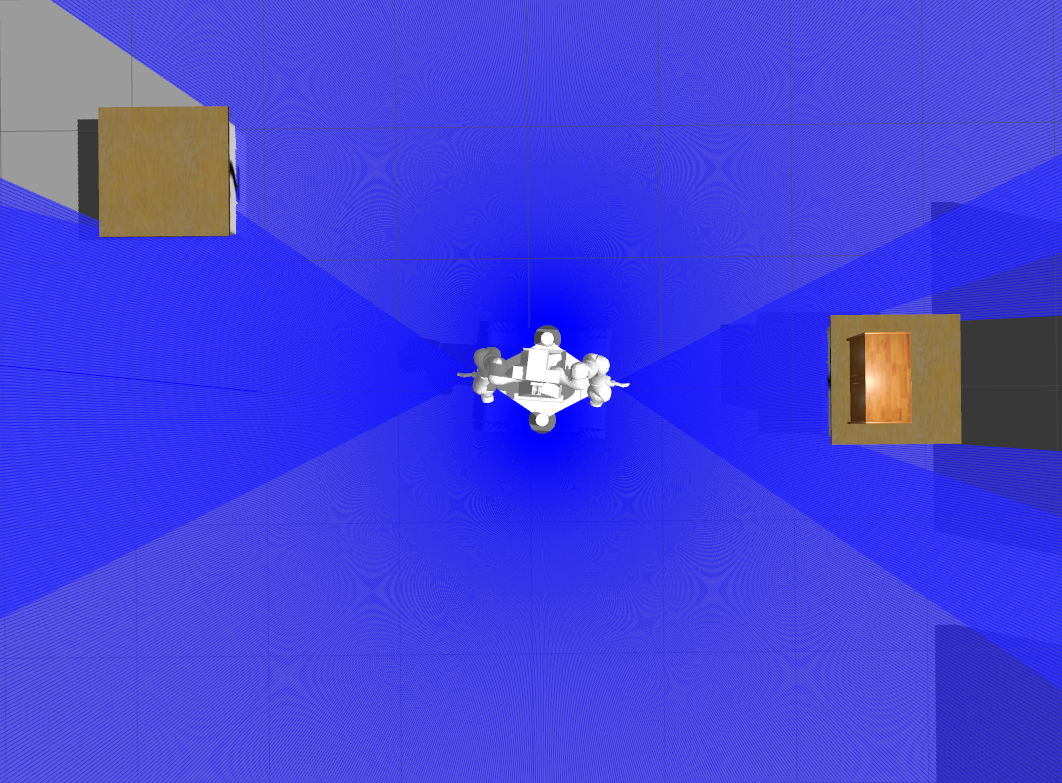
\includegraphics[width=\linewidth]{imgs/wstepne_badania/gazebo_scan.png}
    				\caption{plan globalny i lokalny}
  			\end{subfigure}
  			\begin{subfigure}[h]{\linewidth}
    				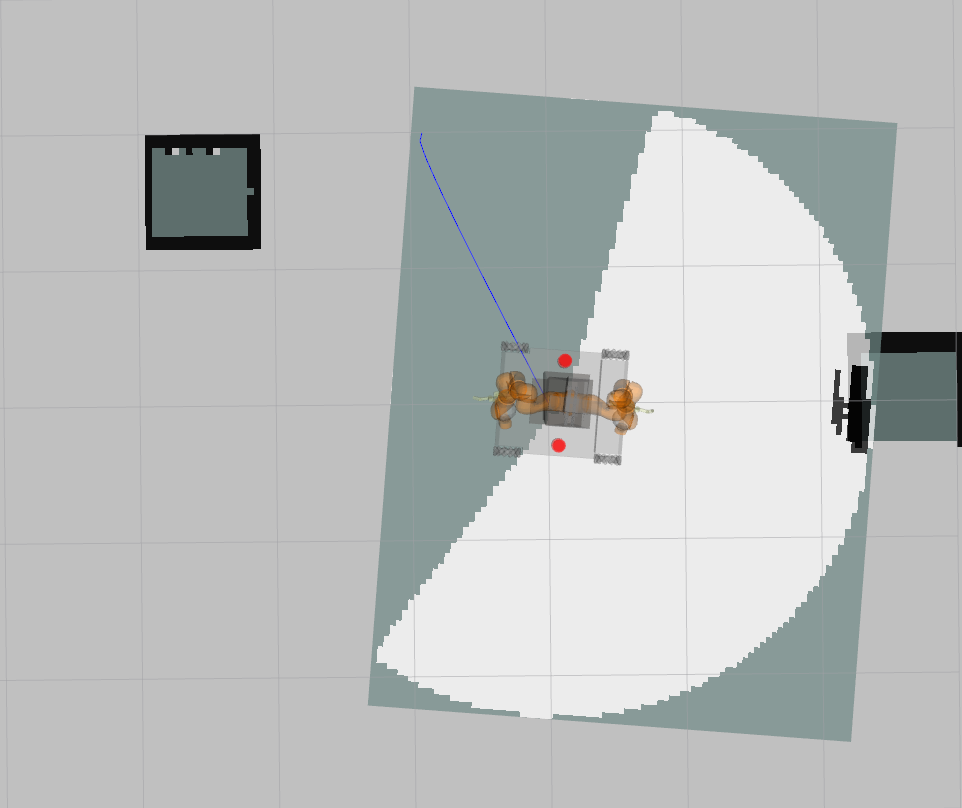
\includegraphics[width=\linewidth]{imgs/wstepne_badania/rviz_scan.png}
   				 \caption{trajektoria ruchu}
  			\end{subfigure}
  			\caption{rzutowanie skanu kamery Kinect}
 			 \label{fig:scan}
		\end{figure}
	
		Na rysunku \ref{fig:mapping} przedstawiono pojedynczy skan laserowy wykonany w nieznanym środowisku przed poruszeniem bazą robota. 

		\begin{figure}[h!]
 			 \centering
  			\begin{subfigure}[b]{0.4\linewidth}
   				 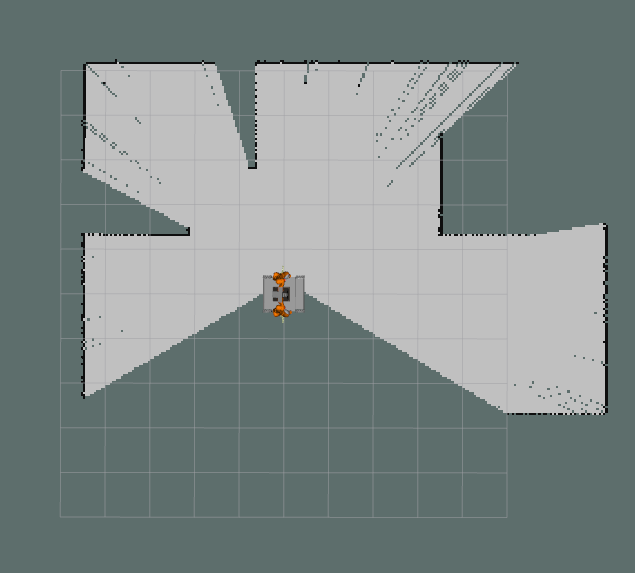
\includegraphics[width=\linewidth]{imgs/wstepne_badania/scan_l.png}
    				\caption{lewy skaner}
  			\end{subfigure}
  			\begin{subfigure}[b]{0.4\linewidth}
    				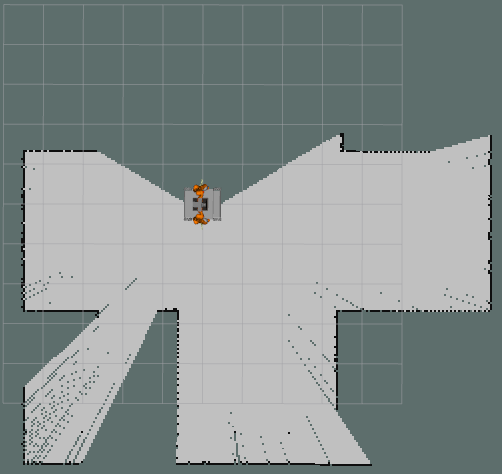
\includegraphics[width=\linewidth]{imgs/wstepne_badania/scan_r.png}
   				 \caption{prawy skaner}
  			\end{subfigure}
			\begin{subfigure}[b]{0.9\linewidth}
    				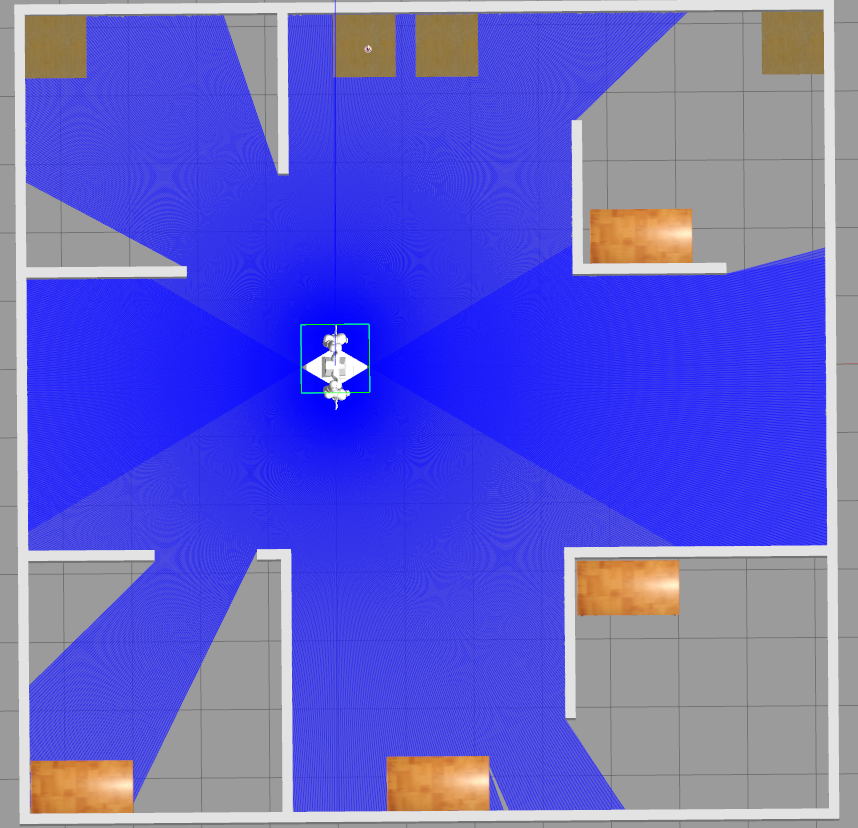
\includegraphics[width=\linewidth]{imgs/wstepne_badania/scan_all.png}
   				 \caption{pokrycie obydwu skanerów}
  			\end{subfigure}
  			\caption{pokrycie przestrzeni}
 			 \label{fig:mapping}
		\end{figure}

	
		Podczas próby przetestowania modułu \textit{gmapping} wykorzystującego pojedynczy skaner laserowy do zbudowania statycznej mapy zajętości okazało się, że w systemie znajdują się błędy uniemożliwiające budowę mapy. 
		Na rysunku \ref{fig:tf} ukazane zostało drzewo transformacji, na którym widać, że pierwotnym układem współrzędnych jest \textit{odom}, z którego następnie jest przeliczana transformacja na układ \textit{world}, a z tego równolegle na \textit{torso\_base} oraz równolegle \textit{map}. 
		Jest to błędna struktura, poprawna posiada \textit{world} jako pierwotny układ współrzędnych, od niego przechodzi transformacja do układu \textit{map}, stąd do \textit{odom}, a wreszcie do \textit{torso\_base}, bez rozgałęzień. 
		
		\begin{figure}
			\centering
			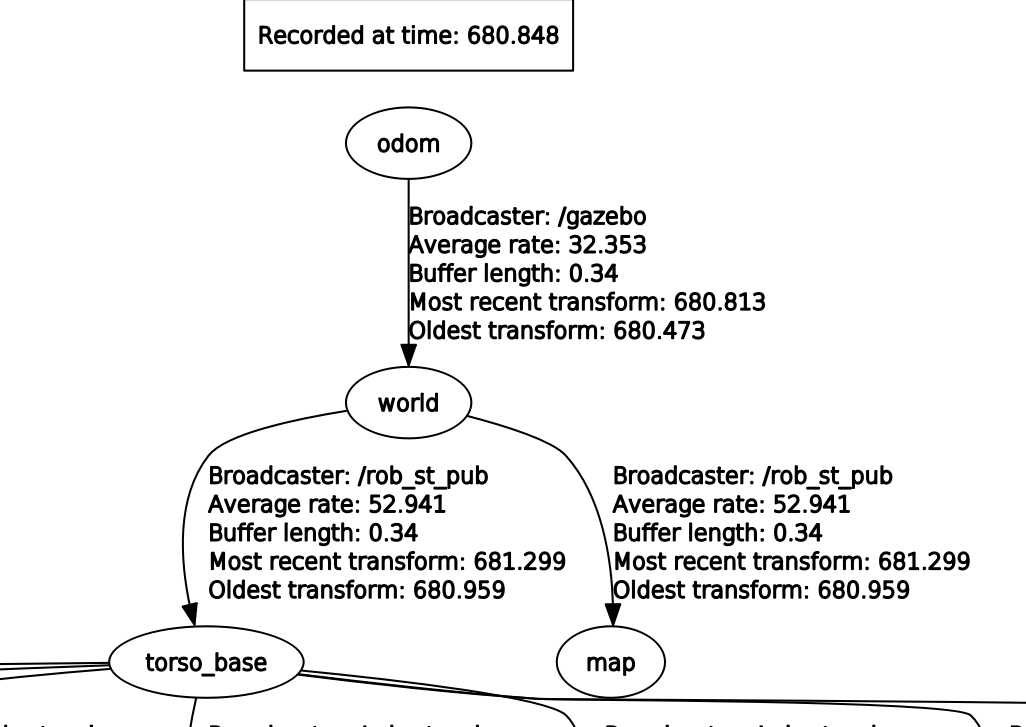
\includegraphics[width=\linewidth]{imgs/wstepne_badania/tf.png}
			\caption{błędne drzewo transformacji}
			\label{fig:tf}
		\end{figure}
		
		
	
	\subsection{lokalizacja}
	
		Ta część badań jest ściśle zależna od budowania mapy oraz poprawności drzewa transformacji.
		Dopóki ten element wykazuje błędne działanie, lokalizacja robota z pomocą odometrii oraz laserów i kamery Kinect, ale też wysyłanie pozycji innych przedmiotów w jego otoczeniu jest niemożliwa.
		Dlatego ta część badań zostaje wstrzymana do czasu usunięcia błędów w drzewie transformacji. 
		Na rysunku ... ukazano próbę jednoczesnej lokalizacji i budowania mapy robota przy opisanym stanie systemu. 
		Robot jechał ze stałą prędkością $0.4$ w kierunku \textit{x} bazy i przejechał w rzeczywistości około $6$ metrów.
		
		\begin{figure}
			\centering
			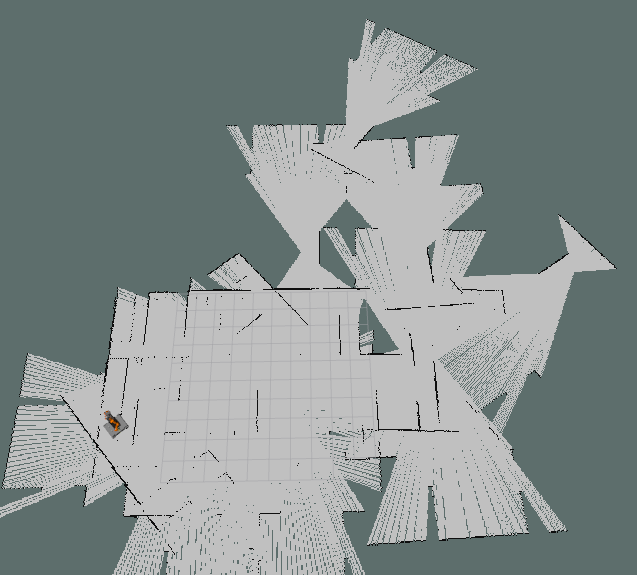
\includegraphics[width=\linewidth]{imgs/wstepne_badania/crazy.png}
			\caption{błąd w dynamicznym tworzeniu mapy statycznej i w lokalizacji}
			\label{fig:tf}
		\end{figure}
		
		
		


%		\begin{figure}[h]
%			\centering
%			\begin{subfigure}[b]{0.4\linewidth}
 %				 \includegraphics[0.8\linewidth]{imgs/wstepne\_badania/plan.png}
%				  \caption{Plan globalny i plan lokalny }
%				  \label{fig:plan}
%			  \end{subfigure}
%			\begin{subfigure}
% 				 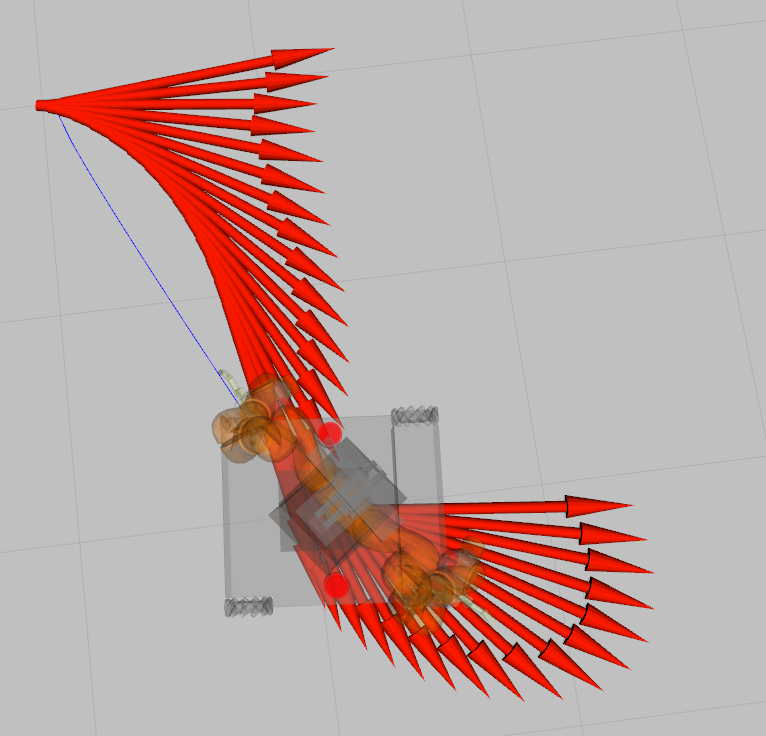
\includegraphics[width=0.8\linewidth]{imgs/wstepne_badania/path.png}
%				  \caption{Plan globalny i plan lokalny }
%				  \label{fig:path}
%			  \end{subfigure}
%		\end{figure}

